\documentclass[10pt,a4paper]{ctexart}
\usepackage[margin=2cm]{geometry}
\usepackage{graphicx}
\usepackage{float}      % 支持 [H] 浮动体选项
\usepackage{hyperref}
\usepackage{amsmath}    % 提供方程环境
\usepackage{physics}    % 简化向量、微分算子语法
\newcommand{\myspace}[1]{\par\vspace{#1\baselineskip}} %自定义空一行
\usepackage{fancyhdr}
\pagestyle{fancy}
\fancyhf{}  % 清除所有页眉页脚
\fancyfoot[C]{\thepage}  % 在页脚中央设置页码
\renewcommand{\headrulewidth}{0pt}  % 去掉页眉横线
\renewcommand{\footrulewidth}{0pt}  % 去掉页脚横线

\usepackage{hyperref}
\hypersetup{
    colorlinks=true,
    linkcolor=blue,
    filecolor=magenta,      
    urlcolor=cyan,
    pdftitle={Overleaf Example},
    pdfpagemode=FullScreen,
    }

\usepackage{titlesec}

% 重新定义section格式
\titleformat{\section}
  {\normalfont\Large\bfseries}
  {\chinese{section}、}
  {0pt}
  {}

% 给出常用字号的自定义指令
\newcommand{\chuhao}{\fontsize{42pt}{48pt}\selectfont}
\newcommand{\xiaochu}{\fontsize{36pt}{42pt}\selectfont}
\newcommand{\xiaoer}{\fontsize{18pt}{21.6pt}\selectfont}
\newcommand{\sanhao}{\fontsize{16pt}{20pt}\selectfont}
\newcommand{\xiaosan}{\fontsize{15pt}{18pt}\selectfont}
\newcommand{\sihao}{\fontsize{14pt}{18pt}\selectfont}
\newcommand{\xiaosi}{\fontsize{12pt}{16pt}\selectfont}
\newcommand{\wuhao}{\fontsize{10.5pt}{12.6pt}\selectfont}

% 定义中文数字转换
\titleformat{\section}
  {\normalfont\Large\bfseries}
  {\zhnum{section}、}  % 使用\zhnum而不是\chinese
  {0pt}
  {}

% 标题设置
\title{\xiaochu\textbf{物理实验报告}}
\author{}
\date{}

\begin{document}

\vspace*{36pt} % 顶部空白

% 居中填写区域
\begin{center}
    
\includegraphics[width = 9cm]{figure/head.png}
    
    \xiaochu\textbf{物理实验报告}
    % 预留空白区域
    \vspace{13pt}
    \vspace{13pt}
    \vspace{13pt}
    \vspace{13pt}
    
    \sanhao\textbf{实验名称：\underline{\makebox[10cm]{ 光的衍射}}} \\[10pt]
    \sanhao\textbf{实验桌号：\underline{\makebox[10cm]{ 9}}} \\[10pt]
    \sanhao\textbf{指导教师：\underline{\makebox[10cm]{姜柏旭 }}} \\[30pt]
    
    % 预留空白区域
    \myspace{6}
    
   \sihao\textbf{班级：\underline{\makebox[6cm]{}}} \\[10pt]
    \sihao\textbf{姓名：\underline{\makebox[6cm]{}}} \\[10pt]
    \sihao\textbf{学号：\underline{\makebox[6cm]{}}} \\[30pt]
    
   \sihao\textbf{实验日期: 
   \underline{\makebox[0.8cm]{2025}}  年 
   \underline{\makebox[0.4cm]{11}}月
   \underline{\makebox[0.4cm]{26}}日  
   星期\underline{\makebox[0.6cm]{三}}上午}
    
    \vspace{18pt}
    \sihao 浙江大学物理实验教学中心
    
\end{center}

\newpage

\section{预习报告}

    \subsection{实验综述}
    
    \xiaosi （自述实验现象、实验原理和实验方法，不超过300字，5分）
 
    \subsubsection{实验原理}

  \begin{enumerate}
    \item \textbf{惠更斯-菲涅尔原理}
    因为同一波前上的各点发出的都是相干子波。而各子波在空间某点的相干叠加，就决定了该点波的强度。
\[
E(P) = \int_s {E_{(p)}} = \int_s F\frac{K(\theta)}{r}\cos(\omega t - \frac{2 \pi r}{\lambda})\d{S}
\]
其中$F$是比例系数，$K(\theta)$为倾斜因子。

    \item \textbf{单缝衍射光强分布特征}
    由菲涅尔原理和矢量振幅法，可知\[
I = I_0 (\frac{\sin \mu}{\mu})^2
\]
想要得到光强度的极值位置，则对$\mu$求偏导
\[
\frac{\partial I}{\partial \mu} = 0
\]
即明纹位置：($a$为狭缝的宽度)
\[
\sin\theta = 0, \pm 1.43\frac{\lambda}{a}, \pm 2.46\frac{\lambda}{a}, \cdots
\]
暗纹位置：
\[
\sin\theta = \pm \frac{\lambda}{a}, \pm \frac{2\lambda}{a}, \cdots
\]
$\pm 1$级明纹的最大光强则为$I_1 \approx 4.7\% I_0$

    \item \textbf{利用光栅衍射法测量激光波长}
    光栅方程（主极大条件）：
\[
d\sin \theta = \pm k\lambda(k = 0, \pm 1, \pm 2, \cdots)
\]
角度较小时，我们有$\sin\theta \approx \tan \theta \approx \frac{x}{D}$，即
\[
x_k = k\frac{D}{d}\lambda
\]
最后由公式\[\frac{x_1 - x_{-1}}{2} \approx \frac{D}{d}\lambda\]
可以求出激光波长

\end{enumerate}

\subsubsection{实验方法}
\begin{enumerate}
    \item \textbf{光路调节与校准：}
    调节光学导轨上的各个光学元件，确保它们的位置共轴且等高，以形成一条清晰、水平的实验光路。

    \item \textbf{观察不同孔隙的衍射图样：}
    将具有不同形状孔隙的衍射板置于光路中，定性观察并记录各自产生的夫琅禾费衍射图样的形状特征。

    \item \textbf{利用一维光栅测定激光波长：}
    精确测量其衍射图样中正一级与负一级主极大亮纹之间的距离，亮纹本身有宽度并且亮纹的界限难以准确判断。

    \item \textbf{研究单缝衍射的光强分布并测量缝宽：}
    观察由单缝产生的夫琅禾费衍射条纹。利用一维光强测量仪测出其光强分布。绘制出相对光强 $I/I_0$ 随位置坐标 $x$ 变化的函数图像，并根据衍射图样中暗纹的位置，计算出该单缝的精确宽度 $a$。

\end{enumerate}
    \myspace{2}
    
    
    \subsection{实验重点}
    
    \xiaosi（简述本实验的学习重点，不超过100字，3分）
    
\begin{enumerate}
    \item \textbf{分析衍射图案：}首先要搞清楚，当光线通过不同形状的物体时，产生的衍射图样的明暗分布有什么不同和规律。
    \item \textbf{准确测量：}准确测量一些光的衍射相关物理量，主要是衍射条纹间距
\end{enumerate}
    \myspace{2}
    
    \subsection{实验难点}
    
    \xiaosi（简述本实验的实现难点，不超过100字，2分）

\begin{enumerate}
    \item 实验开始前需要调整光学导轨，确保各光学元件等高且共轴
    \item 转动轮毂时只能单向转动
    \item 测准确测量衍射条纹间距
\end{enumerate}
\myspace{2}
\section{原始数据}

    \xiaosi （将有老师签名的“自备数据记录草稿纸”的扫描或手机拍摄图粘贴在下方，20分）
   

 \begin{figure}[H]
    \centering
    
\includegraphics[width=0.9\textwidth]{figure/raw_data.jpg}
    \caption{光的衍射原始数据记录}
\end{figure}
\section{结果与分析}

    \subsection{数据处理与结果}
    \xiaosi （列出数据表格、选择数据处理方法、给定测量或计算结果，30分）

    \subsubsection{利用光栅衍射测量激光波长}
    \begin{table}[H]
\centering
\caption{利用光栅衍射法测量光的波长数据记录表}
\label{tab:lambda}
% \resizebox{\textwidth}{!}{%
\begin{tabular}{|ll|ll|}
\hline
\multicolumn{1}{|l|}{序号} & $x_{+1}(mm)$ & \multicolumn{1}{l|}{$x_{-1}(mm)$} & $\lambda$                        \\ \hline
\multicolumn{1}{|l|}{1} & 69.779 & \multicolumn{1}{l|}{38.633} & 622.9 \\ \hline
\multicolumn{1}{|l|}{2} & 68.520 & \multicolumn{1}{l|}{38.633} & 637.7 \\ \hline
\multicolumn{1}{|l|}{3} & 68.520 & \multicolumn{1}{l|}{37.519} & 620.0 \\ \hline
\multicolumn{1}{|l|}{4} & 69.609 & \multicolumn{1}{l|}{37.519} & 641.8 \\ \hline
\multicolumn{1}{|l|}{5} & 69.609 & \multicolumn{1}{l|}{37.474} & 642.7 \\ \hline
\multicolumn{1}{|l|}{6} & 68.725 & \multicolumn{1}{l|}{37.474} & 625.0 \\ \hline
\end{tabular}%
% }
\end{table}
波长根据公式$$ \lambda = d \sin \theta = \frac{d \Delta x}{2 \Delta L} $$
计算，其中$d =  0.02  mm$，$\Delta L = 50.00 cm$，$\Delta x = |x_{+1} - x_{-1}|$。
波长平均值：
$$ \overline{\lambda} = \frac{1}{6} \sum_{i=1}^{6} \lambda_i = \frac{622.9 + 637.7 + 620.0 + 641.8 + 642.7 + 625.0}{6} =631.5\, \text{nm}$$

先计算各次测量的残差及其平方：

\begin{align*}
v_1 &= 622.9 - 631.5 = -8.6, &\quad v_1^2 = 73.96 \\
v_2 &= 637.7 - 631.5 = 6.2, &\quad v_2^2 = 38.44 \\
v_3 &= 620.0 - 631.5 = -11.5, &\quad v_3^2 = 132.25 \\
v_4 &= 641.8 - 631.5 = 10.3, &\quad v_4^2 = 106.09 \\
v_5 &= 642.7 - 631.5 = 11.2, &\quad v_5^2 = 125.44 \\
v_6 &= 625.0 - 631.5 = -6.5, &\quad v_6^2 = 42.25
\end{align*}

残差平方和：
$$ \sum_{i=1}^{6} v_i^2 = 73.96 + 38.44 + 132.25 + 106.09 + 125.44 + 42.25 = 518.43 $$

单次测量的标准偏差：
$$ s(\lambda) = \sqrt{\frac{\sum_{i=1}^{6} v_i^2}{n-1}} = \sqrt{\frac{518.43}{5}} = \sqrt{103.686} = 10.183 \, \text{nm} $$


根据A类不确定度公式：
$$ u_A(\bar{\lambda}) = \frac{s(\lambda)}{\sqrt{n}} = \frac{10.183}{\sqrt{6}} = \frac{10.183}{2.44949} = 4.156 \, \text{nm} $$

取两位位有效数字：
$$ u_A(\bar{\lambda}) = 4.2 \, \text{nm} $$
因此，激光
波长测量结果的A类不确定度为：
$$ \boxed{u_A(\bar{\lambda}) = 4.2 \, \text{nm}} $$

对应的相对不确定度为：
$$ \frac{u_A(\bar{\lambda})}{\bar{\lambda}} = \frac{4.16}{631.5} \times 100\% = 0.66\% $$

波长最终测量结果为：
$$ \lambda = (631.5\pm 4.2) \, \text{nm} $$

波长测量相对误差为：
$$ \frac{650.0-631.5}{650.0}=2.8 \% $$

\subsubsection{利用单缝衍射测出狭缝宽度}
\begin{table}[H]
\centering
\caption{利用单缝衍射测狭缝宽度数据记录表}
\label{tab:a}
\begin{tabular}{|l|l|l|l|}
\hline
序号 & $x_{+1}(\mathrm{mm})$ & $x_{-1}(\mathrm{mm})$ & $a(\mu\mathrm{m})$ \\
\hline
1 & 57.639 & 45.579 & 74.88 \\
2 & 57.632 & 45.503 & 74.45 \\
3 & 57.632 & 45.265 & 73.01 \\
4 & 57.715 & 45.265 & 72.53 \\
5 & 57.709 & 45.013 & 71.11 \\
6 & 57.709 & 45.139 & 71.84 \\
\hline
\end{tabular}
\end{table}

由单缝衍射一级亮纹的位置$\sin \theta = \pm 1.43 \frac{\lambda}{a}$，且$\sin \theta \approx \theta \approx \tan \theta = \frac{\Delta x}{2\Delta L}$，其中$\Delta L = 50.00\,\mathrm{cm}$，$\lambda = 631.5\,\mathrm{nm}$，得出
\[
a = \frac{1.43 \cdot 2 \Delta L\lambda}{\Delta x}
\]
其中$\Delta x = |x_{+1} - x_{-1}|$。

计算各组的$a$值如上表。则$a$的平均值为：
\[
\bar{a} = \frac{74.88 + 74.45 + 73.01 + 72.53 + 71.11 + 71.84}{6} = 72.97 \, \mu\mathrm{m}
\]

A类不确定度计算：先计算标准偏差$s$，
\[
s = \sqrt{\frac{\sum_{i=1}^{6} (a_i - \bar{a})^2}{6-1}} = 1.47 \, \mu\mathrm{m}
\]
则
\[
u_A = \frac{s}{\sqrt{n}} = \frac{1.47}{\sqrt{6}} = 0.60 \, \mu\mathrm{m}
\]
修约后，不确定度保留一位有效数字，$u_A = 0.6 \, \mu\mathrm{m}$，平均值修约到与不确定度对齐，$\bar{a} = 73.0 \, \mu\mathrm{m}$。

最终狭缝宽度为：
\[
a = (73.0 \pm 0.6) \, \mu\mathrm{m}
\]
    \myspace{2}
\subsubsection{绘制单缝衍射中光强分布}
从-2级暗纹到+2级暗纹中，每{0.400}{mm}测量一次光强，绘制出光强(光电流)随位置坐标$x$变化的函数图像，如所示。
\begin{figure}[H]
    \centering
    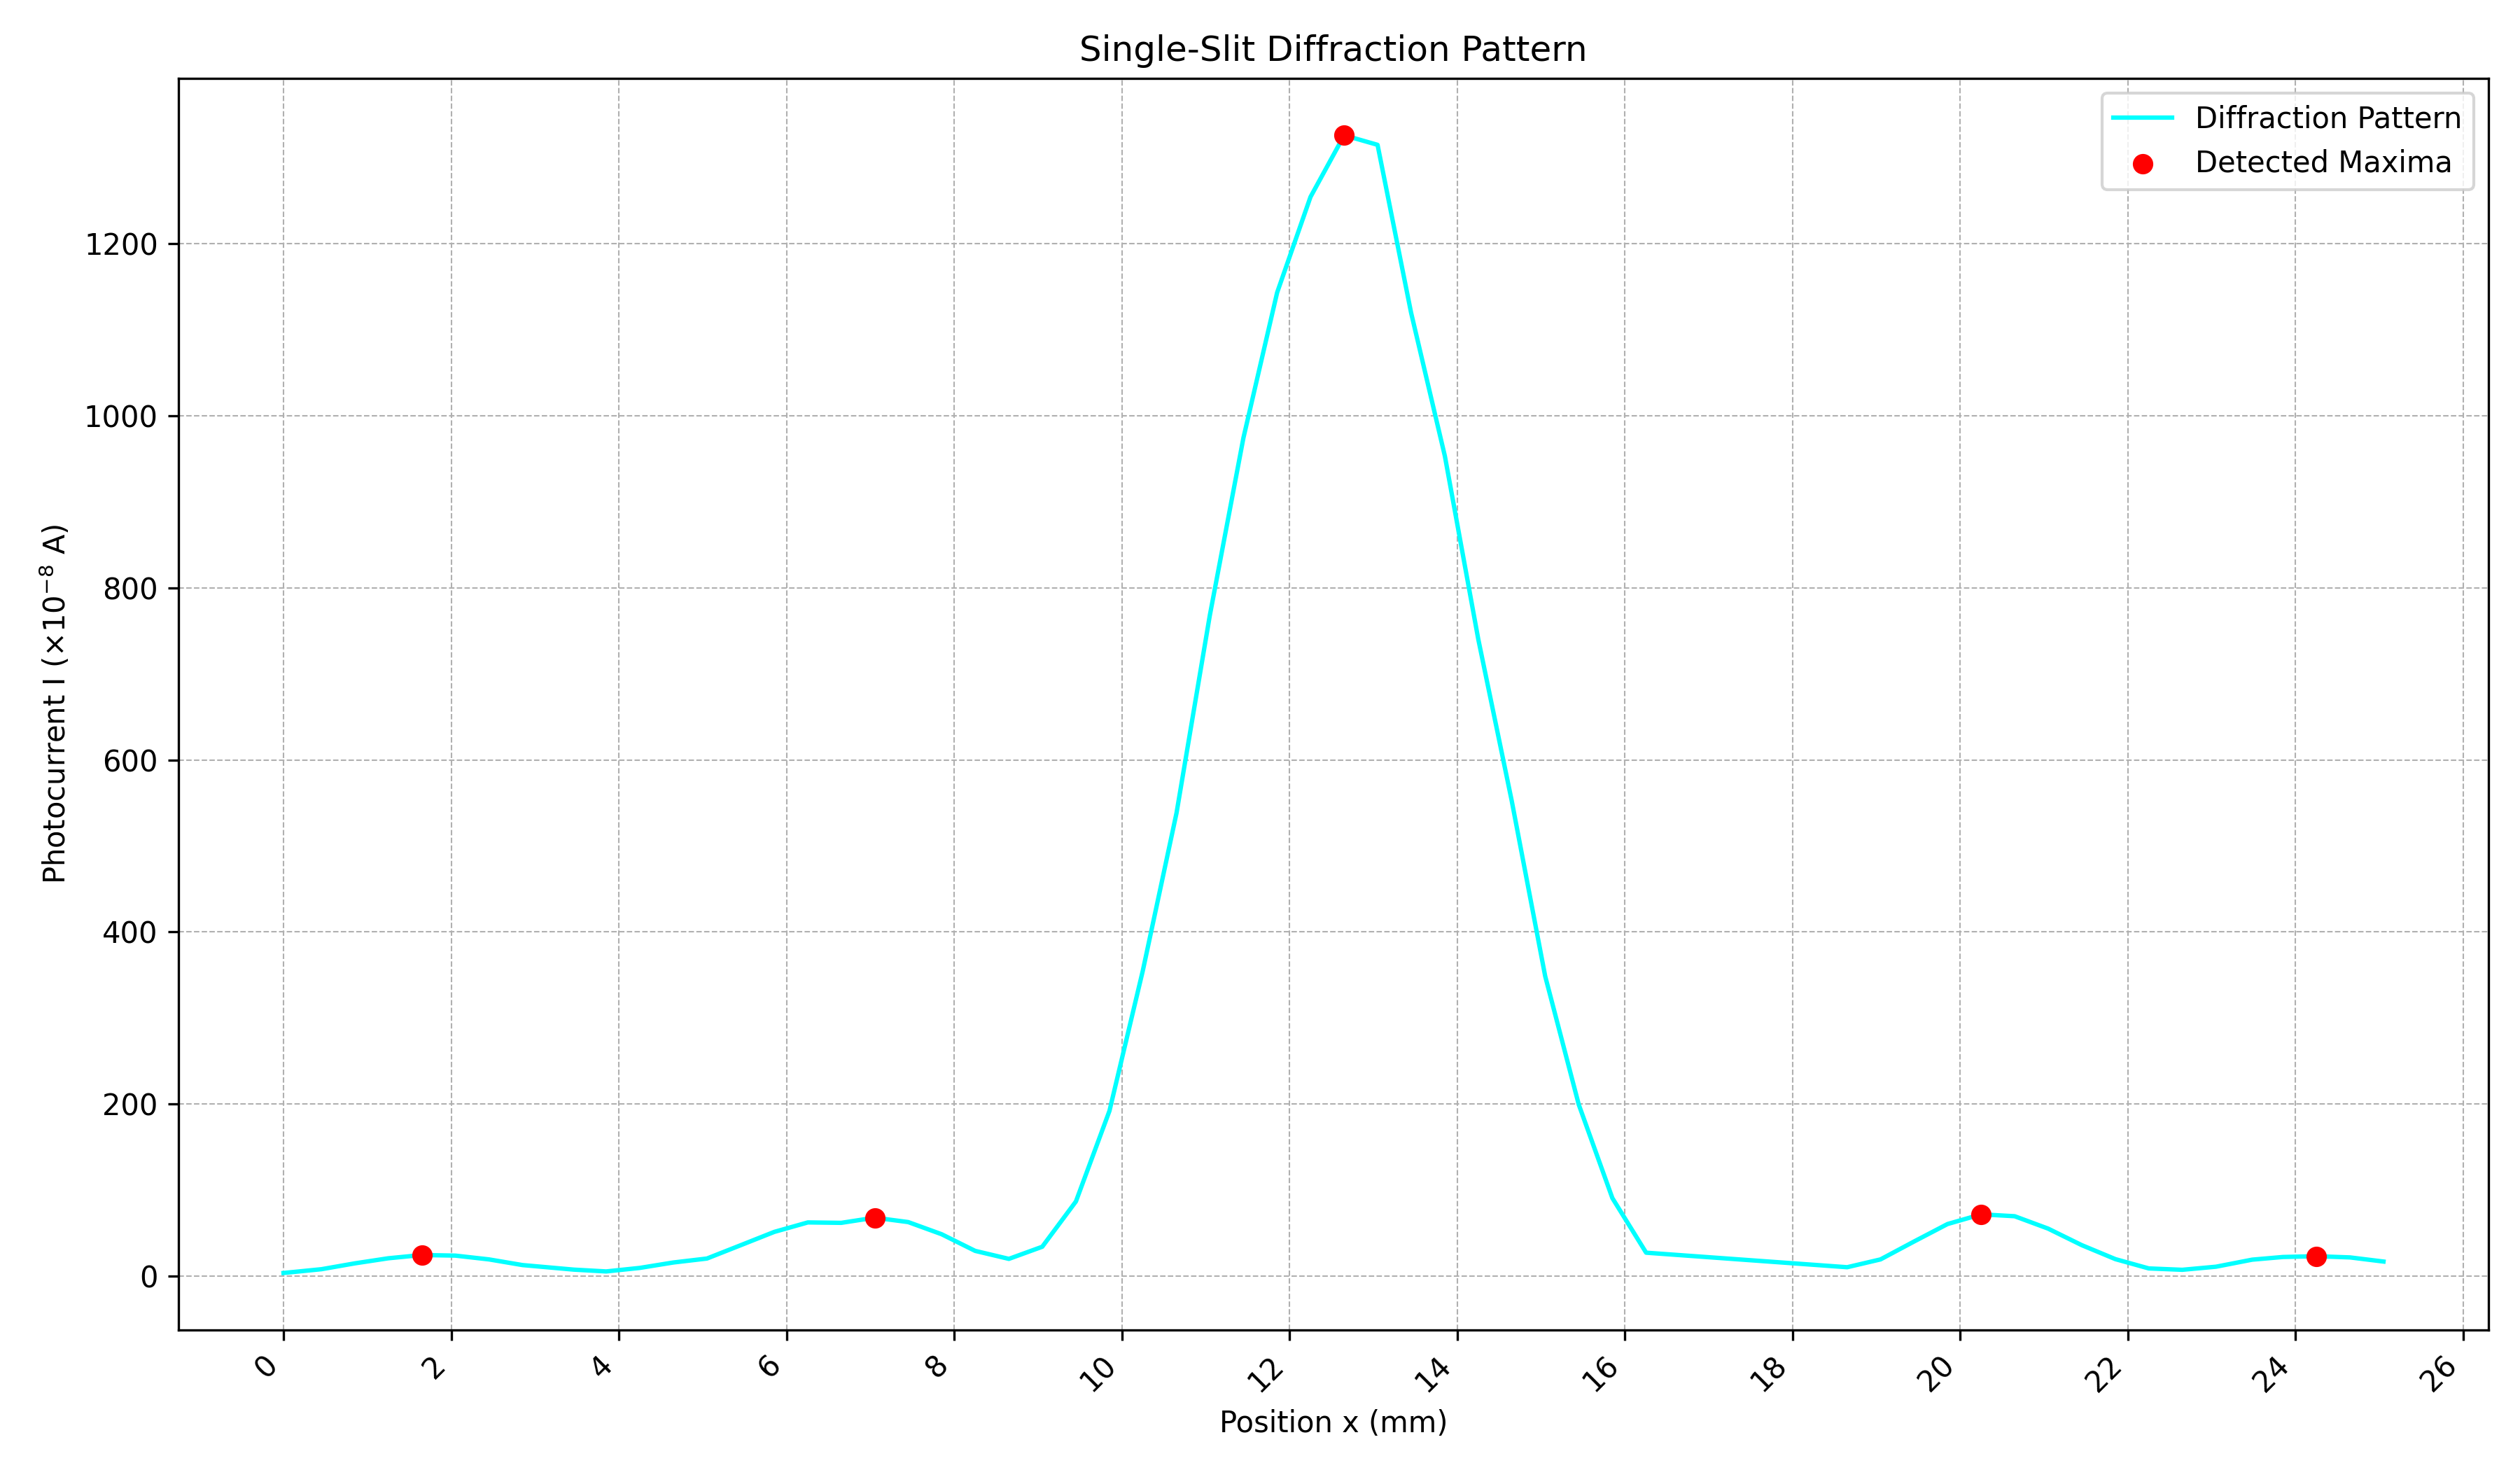
\includegraphics[width=.7\textwidth]{figure/figure.png}
    \caption{单缝衍射中光强分布图像}
    \label{fig:intensity}
\end{figure}

\subsubsection{验证光强公式}
测得0级亮纹的最大光强是$I_0 = 1326.3 \times 10^{-8}A$， 一级亮纹的亮度是$I_1 = 69.7 \times 10^{-8}A$
\[
\frac{69.7 \times 10^{-8}}{1326.3 \times 10^{-8}} = 5.3\% \approx 4.7\%
\]
符合理论预期。
    \subsection{误差分析}
    \xiaosi （运用测量误差、相对误差、不确定度等分析实验结果，20分）

    本实验的主要误差来源包括：

1. \textbf{系统误差}：

光学元件共轴调节不完美导致的测量偏差

测微目镜的零点误差和回程差

小角度近似$\sin\theta \approx \tan\theta$引入的理论误差

激光器波长稳定性（约$\pm 1,\mathrm{nm}$）

2. \textbf{随机误差}：

条纹位置判读误差，特别是条纹边缘模糊时的主观判断误差

仪器读数误差，估计为$\pm 0.005,\mathrm{mm}$

环境振动和空气扰动对光路的影响

3. \textbf{波长测量误差分析}：

相对误差$2.8\%$，相对不确定度$0.66\%$

主要来源于光栅常数$d$的标称误差和距离$D$的测量误差

4. \textbf{缝宽测量误差分析}：

主要受限于衍射条纹的清晰度和位置判读精度

5. \textbf{光强测量误差分析}：
光电流测量仪的灵敏度和线性范围限制.光电流测量仪读数不稳定。

总体而言，实验结果与理论预期符合较好，验证了光的衍射理论。

    \subsection{实验探讨}
    \xiaosi （对实验内容、现象和过程的小结，不超过100字，10分）

    通过本实验，深入理解了光的衍射现象及其规律。单缝衍射图样呈现明暗相间的条纹分布，中央明纹最宽最亮；光栅衍射则产生分立的尖锐谱线。实验验证了衍射理论公式，掌握了光学精密测量技术。
    验证了单缝衍射的光强分布公式，测量了激光波长和狭缝宽度，结果与理论值较为接近。
    实验培养了严谨的科学态度和细致的操作技能。
\section{思考题}

    \xiaosi （解答教材或讲义或老师布置的思考题，10分）

1.单缝衍射两侧光强不是严格对称的原因是什么（主要因素即可）？

主要原因包括：激光光束强度分布不均匀；单缝边缘可能存在微小瑕疵或污染；光学元件未严格共轴；接收屏或光强探测器位置有微小倾斜。这些因素会导致衍射图样左右不对称。

2.狭缝太宽或太窄会发生什么情况，为什么？

狭缝太宽时，衍射角变小，条纹密集难以分辨，趋向于几何光学现象；狭缝太窄时，透过光强过弱，条纹模糊不清，且可能因缝宽与波长可比而出现更复杂的衍射效应。最佳缝宽应使衍射条纹清晰可辨且光强适中。

3.光栅衍射时会发生缺级现象，为什么？

缺级现象发生在光栅衍射主极大与单缝衍射极小重叠时。当满足$d\sin\theta = k\lambda$（光栅方程）和$a\sin\theta = k'\lambda$（单缝衍射极小条件）同时成立时，该级主极大消失。这是因为单缝衍射的包络线调制了光栅衍射的强度分布。

4.在衍射的障碍物为圆屏时，无论圆屏的尺度有多大（在能够观察到衍射图样的范围内），衍射图样的中心总是会有一个亮斑，请解释这个现象发生的原因。（选答，根据答案酌情加分）

这是泊松亮斑现象。根据菲涅尔衍射理论，圆屏边缘各点作为次波源，发出的子波在圆屏几何阴影中心处相干叠加。由于圆对称性，这些子波到达中心的光程差为零，干涉相长，因此在阴影中心形成亮斑。这一现象有力地支持了光的波动说。
\newpage

\sihao\textbf{注意事项：}
\xiaosi
\begin{enumerate}
    \item 用PDF格式上传“实验报告”，文件名：学生姓名+学号+实验名称+周次。
    \item  “实验报告”必须递交在“学在浙大”的本课程的对应实验项目的“作业”模块内。
    \item  “实验报告”成绩必须在“浙江大学物理实验教学中心网站”-“选课系统”内查询。
    \item 教学评价必须在“浙江大学物理实验教学中心网站”-“选课系统”内进行，学生必须进行教学评价，才能看到实验报告成绩，教学评价必须在本次实验结束后 3 天内进行。
\end{enumerate}

\vspace{1cm}
\xiaosi\centering \textbf{浙江大学物理实验教学中心制}

\end{document}